% +------------------------------------------------------------------------+
% | Reference manual page: intro.tex
% +------------------------------------------------------------------------+
% | 09.02.2006   Marc Pouget and Fr�d�ric Cazals
% | Package: Jet_fitting_3
% | 
\RCSdef{\RCSintroRev}{$Id$}
\RCSdefDate{\RCSintroDate}{$Date$}
% |
%%RefPage: end of header, begin of main body
% +------------------------------------------------------------------------+

\ccRefChapter{Estimation of Local Differential Properties of Sampled
Surfaces via Polynomial Fitting}
\label{ref_chap:Jet_fitting_3}
  
\ccChapterAuthor{Marc Pouget \and Frederic Cazals}

\subsection*{Introduction}

The following picture illustrates the template dependencies.
\begin{figure}[h!]
\begin{ccTexOnly}
\centerline{
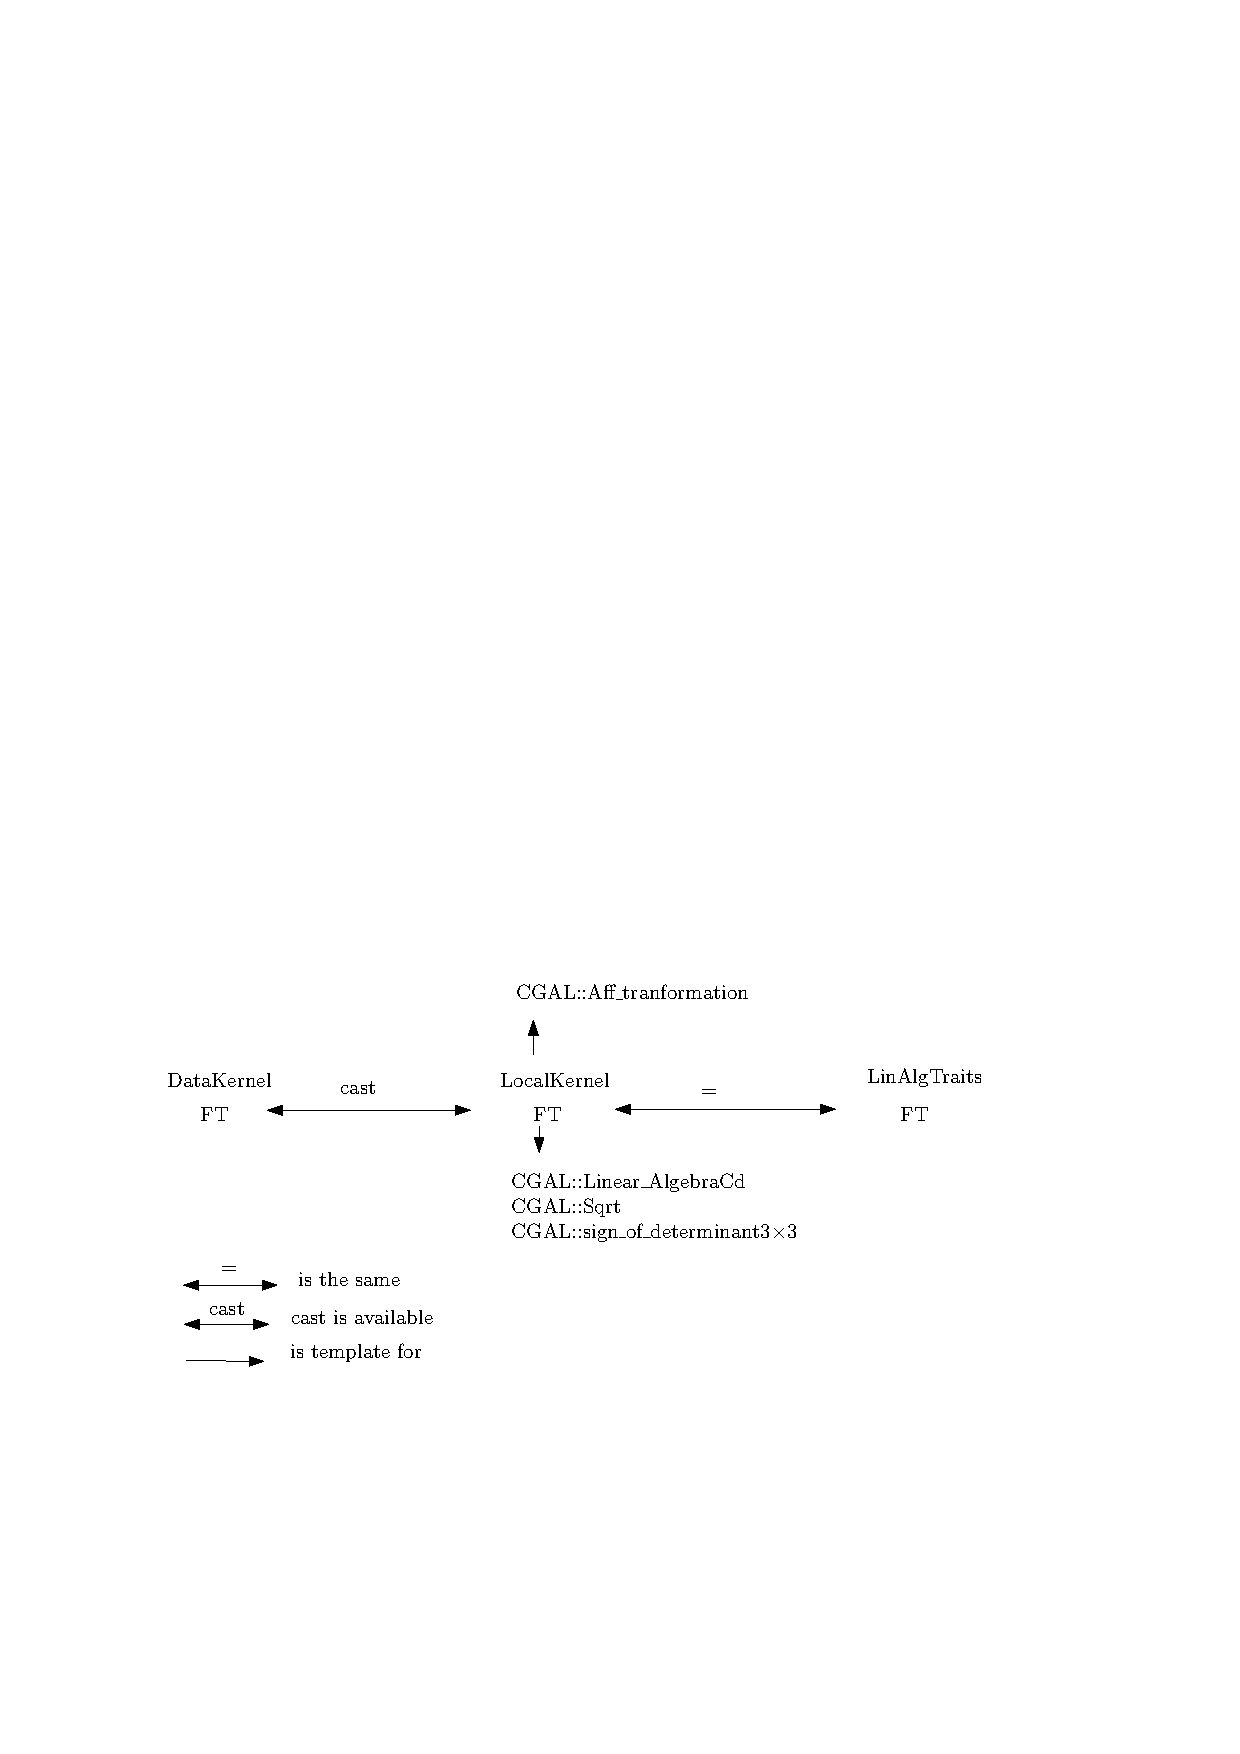
\includegraphics[width=.5\linewidth]{Jet_fitting_3_ref/template_dependence}}
\end{ccTexOnly}

\label{fig:template_dependence}
%\caption{}

\begin{ccHtmlOnly}
<CENTER>
<img border=0 src="template_dependence.jpg" width=600>
</CENTER>
\end{ccHtmlOnly}
\end{figure}


\ccRequirements
The three classes  \ccc{Monge_rep}, \ccc{Monge_info} and
\ccc{Monge_via_jet_fitting} are designed to be used
simultaneously. 

The \ccc{DataKernel} template parameter must be the
same for the classes \ccc{Monge_rep} and
\ccc{Monge_via_jet_fitting}. The \ccc{LocalKernel} template parameter
must be the same for the classes \ccc{Monge_info} and
\ccc{Monge_via_jet_fitting}. 

\subsection*{Concepts}
\ccRefConceptPage{DataKernel} \\
\ccRefConceptPage{LocalKernel} \\
\ccRefConceptPage{LinAlgTraits} \\

\subsection*{Classes}
\ccRefIdfierPage{CGAL::Monge_rep<DataKernel>}\\
\ccRefIdfierPage{CGAL::Monge_info<LocalKernel>}\\
\ccRefIdfierPage{CGAL::Monge_via_jet_fitting<DataKernel,LocalKernel,LinAlgTraits>}\\

% +------------------------------------------------------------------------+
%%RefPage: end of main body, begin of footer
% EOF
% +------------------------------------------------------------------------+

